\subsection{PeerManager}\label{sec:mit-peerManager}

As the name suggests, the \lstinline|PeerManager| is the component that keeps track of all peers known to the current node. The representation of these peers is called \lstinline|RemotePeer|. Through the PeerManger, other components can obtain all known RemotePeers, connect to new RemotePeers and destroy existing RemotePeers. Also, messages are send via the PeerManager.

\paragraph{Obtaining RemotePeers} \label{paragraph:obtain-remotepeers}
Existing RemotePeers can be obtained through the PeerManager. Instances are returned in a \lstinline|TableView| so the result can be filtered and sorted. The filter and sort operations do not affect the internal state of the peer manager because the TableView is exposed as a clone. 

By implementing the \textit{observer} software pattern, other components can subscribe on \textit{PeerChurn}. \textit{PeerChurn} means that subscribers are notified about \lstinline|Added| or \lstinline|Removed| peers so they can act accordingly.

\paragraph{Connect to a RemotePeer}
Through a given address the PeerManager can create a new RemotePeer and establish a connection. The connection can be either a direct connection which means a physical connection or a virtual connection. A virtual connection is \say{opened} for RemotePeers, that are addressable via another direct RemotePeer. This happens when a peer receives a message where the sender is not a direct peer.

\paragraph{Handle Incoming Messages}
\begin{itemize}
    \itembf{Connection negotiation} Incoming \connectionNegotiation messages are handled by the PeerManager. When an offer arrives, it makes sure that a new WebRTC connection is created with an answer for the offer. An incoming answer is used to establish the connection.
    \itembf{Router alive} When an alive message is received from a router, the PeerManager updates the score of all directly connected RemotePeers.
    \itembf{Peer update} RemotePeers that are announced via a peer update are either added to the RemotePeer table or updated, if they were already known.
\end{itemize}

\paragraph{Destroy a RemotePeer}
The PeerManager has the power to destroy a RemotePeer. In this process all connections to the RemotePeer are closed. 
Destroying a peer can either happen explicitly by calling the \lstinline|removePeer(remotePeer)| method or implicitly when the PeerManager notices that a RemotePeer does not have any open connections anymore.

Also, it monitors direct connections that are bound to a virtual connection. When a direct connection is closed and there is no other open direct connection, the PeerManager also closes the virtual connection.

\begin{figure}
  \centering
    \subfloat[]{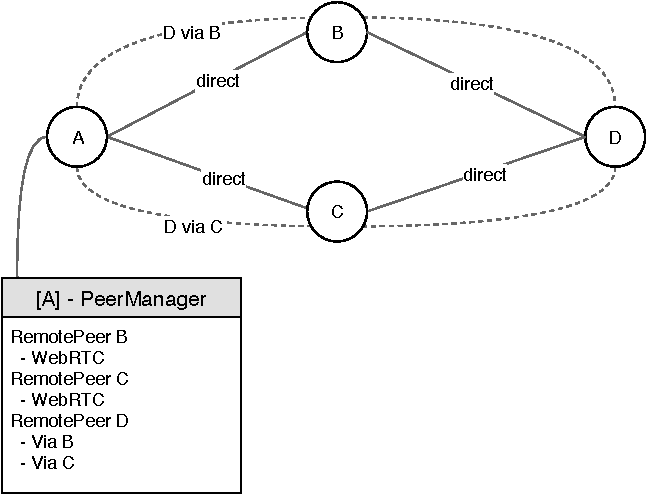
\includegraphics[width=0.4\textwidth]{graphics/implementation/mitosis-peer-manager.pdf} \label{fig:peer-manager-a}}
    \hspace{1 cm}
    \subfloat[]{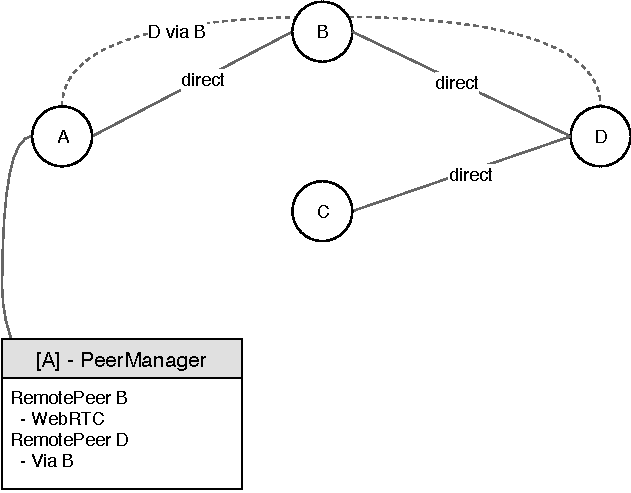
\includegraphics[width=0.4\textwidth]{graphics/implementation/mitosis-peer-manager-2.pdf} \label{fig:peer-manager-b}}
	\caption{PeerManager RemotePeer table}
\label{fig:peer-manager}
\end{figure}

\vref{fig:peer-manager} shows how the RemotePeer table of Mitosis node \textit{A} would look like for the given connection state. \vref{fig:peer-manager-b} shows how the PeerManager is cleaning up RemotePeers and connections after loosing its connection to Mitosis node \textit{C}. 

\paragraph{Send a message}
Sending a message to a remote peer is also initiated through the PeerManager. As each peer has a quality, which is described further in \vref{sec:mit-peer-meter}, the PeerManager is selecting the optimal routing path for the message based on the quality of its peers.
